\documentclass[a4paper,10pt]{article}
\usepackage{mathtext}
\usepackage[T2A]{fontenc}
\usepackage[utf8x]{inputenc}
\usepackage[english,ukrainian]{babel}
\usepackage{amsfonts,amsmath,stmaryrd}
\usepackage{indentfirst}
\usepackage[pdftex]{color,graphicx}

\DeclareGraphicsRule{.jpeg}{.bmp}{}{}
\textwidth 16 cm
\textheight 24.5cm
\topmargin -1 cm
\evensidemargin 0 cm
\oddsidemargin 0 cm

%opening
\title{Індуктивні методи моделювання навігації агента}
\author{Накрийко Андрій}

\begin{document}
\selectlanguage{ukrainian}
\maketitle

\begin{abstract}

\end{abstract}

\section{Вступ}
\section{Проблема керування}
\section{Експертні правила та штучна нейронна мережа}
Першим підходом до розв'язання задачі керування агентом було використання нейромережі з певним наперед заданим набором експертних правил. Ідея такого підходу полягає в тому, щоб, задавши набір ключових правил, використати здатність нейромережі до генералізації даних і поширити експертні знання на увесь простір можливих ситуацій. Таким чином, можна отримати контролер, який здатний приймати ``осмислені'' рішення в ситуаціях, для яких не було надано експертних правил, на основі правил, заданих для ``близьких'' ситуацій.
\subsection{Результати підходу на основі експертних знань}

Результати не можна охарактеризувати однозначно. З однiєї сторони, система контролю на базi нейромережi досить адекватно керувала автомобiлем з доволі складною фізикою, успiшно оминаючи перешкоди та забезпечуючи безперервний рух автомобiля в середовищi, про яке вона не мала жодної попередньої iнформацiї. Бiльше того, для пiдвищення рiвня “природностi” керування, системi контролю надавалася лише iнформацiя про об’єкти, якi попадали в поле зору автомобiля, що являло собою сектор з визначеним радiусом (дальнiстю бачення) та центральним кутом (кутом огляду). Базуючись лише на даних про вiддаль до найближчих об’єктiв в полi зору, система контролю забезпечувала завчасне оминання перешкоди з плавною змiною швидкостi та напрямку руху автомобiля. Очевидно, що велику роль в досягненнi вказаної природностi та адекватностi керування вiдiграла вдало пiдiбрана навчальна множина.

З iншого боку, найбiльшою проблемою, з якою довелося зiткнутися, була наявнiсть ситуацiй, в яких автомобiль зупинявся i система контролю не могла вивести його з нерухомого стану. Це, зокрема, ситуацiя, подана на рис.~\ref{car_stuck}, в якiй автомобiль заїхав у глухий кут i застряг, не зумiвши здiйснити розворот назад. Цю проблему, теоретично, можна було б розв'язати, ввівши у визначення стану автомобіля значення поточної швидкості та задавши додаткові набори ключових експертних правил, які б дозволили автомобілю здійснити розвертання у разі застрягання в глухому куті. Проте на практиці це достатньо проблематично, оскільки введення додаткової змінної стану призводить до ускладення поведінки всієї системи, підвищення рівня вимог до точності та репрезентативності експертних правил. Більше того, для того, щоб зробити розвертання автомобіля безпечнішим та природнішим, довелося б вводити також змінні, які б відповідали за задній огляд автомобіля, що призводить до ще більш строгих вимог до експертних правил.

Слiд зазначити, що ще однiєю причиною (окрiм вказаної обмеженостi визначеного стану динамiчної системи) такої поведiнки є особливiсть фiзичної моделi автомобiля. Мається на увазi природа автомобiля "--- для того щоб здiйснити поворот, чи, тим бiльше, розворот, автомобiль повинен здiйснювати поступальний рух, що в умовах, коли вже вiдбулося ``застрягання'', дуже проблематично. Можливим розв’язанням даної проблеми є змiна типу транспортного засобу. Якщо взяти транспортний засiб, здатний здiйснювати поворот без поступального руху, то можна значно зменшити ймовiрнiсть його застрягання. Таким транспортним засобом, для прикладу, може бути танк, в якому шляхом незалежного обертання гусениць
в рiзнi сторони можна домогтися розвороту на будь-який кут, стоячи при цьому на мiсцi.

Ще однією важливою проблемою є вибір внутрішньої структури нейромережі. Якщо використати недостатню кількість нейронів, то нейромережа не зможе в достатній мірі вивчити набір правил і, таким чином, не зможе в повністю використати експертні знання. З іншого боку, використовуючи надто велику кількість нейронів, існує загроза надто точного запам'ятовування (overfitting) правил без належної генералізації їх на схожі ситуації. В такому випадку нейромережа буде точно виконувати задані правила у відповідних ситуаціях, але навіть незначна зміна ситуації призведе до різкої зміни значень керованих змінних, порівняно з близькою еталонною ситуацією.

Таким чином, при використанні наперед заданих експертних правил, з'являється велика кількість практичних питань, на які немає чітких теоретичних відповідей, а все доводиться вирішувати в результаті численних експериментів. Саме тому було вирішено відійти від підходу, який базується на заздалегідь відібраних експертних знаннях, а піти шляхом самоорганізації "--- дати можливість агенту розробити власну систему правил на основі отриманого внаслідок взаємодії з середовищем досвіду.

\section{Самоорганізаційний підхід "--- навчання з підсиленням}

Оскільки використання попереднього підходу сильно залежить від якості навчальної вибірки (експертних правил), що при найменшому ускладненні сприйняття агентом середовища призводить до значних ускладнень експертних правил, було вирішено відійти від моделі навчання з учителем. Натомість був використаний самоорганізаційний підхід. Основна ідея такого підходу полягає в тому, щоб дати можливість агенту розробити власну систему правил щодо оптимальної поведінки в умовах середовища, завдяки безпосередній взаємодії з середовищем. Взаємодіючи з середовищем, агент отримує певний досвід і, якщо задати певний механізм оцінки агентом власних дій, то в результаті достатньої кількості ``досвіду'', можна надіятися, що агент розробить ефективну стратегію поведінки. Такий підхід отримав назву \emph{навчання з підсиленням (reinforcement learning)}. При використанні навчання з підсиленням відпадає необхідність в досить складному і трудомісткому процесі розробки системи якісних і репрезентативних експертних правил, хоча, натомість, з'являєть необхідність в виборі механізму оцінки дій агента. Проте, для достатньо складних систем зазвичай значно легше визначити механізм оцінки дій, аніж розробити достатньо повну та якісну систему правил.

Ми розглянемо застосування такого індуктивного процесу навчання (на відміну від дедуктивного на базі системи правил) до вищезазначеної задачі навігації агента в умовах наперед не відомого середовища, використавши принцип навчання з підсиленням (reinforcement learning).

\subsection{Загальні поняття навчання з підсиленням}

Ідея навчання з підсиленням полягає в наступному. Існує дві сутності "--- середовище та агент, що діє у ньому. Агент певним чином здатний сприймати середовище та має набір можливих дій, якими він здатний змінювати середовище. Уся сукупність інформації, доступна агенту в кожен дискретний момент часу $t$, називається \emph{станом} і позначається $s_t$. Відповідно можна ввести поняття множини усіх можливих станів середовища $\mathcal{S}\ (s_t \in \mathcal{S})$. Слід зазначити, що множина можливих станів може бути як дискретною, так і неперервною, а отже і нескінченною. При цьому в більшості реальних застосувань множина станів нескінченна. Також визначимо множину \emph{дій} агента, які допустимі в стані $s_t$ "--- $\mathcal{A}(s_t)$. Множина допустимих дій також в загальному випадку може бути нескінченною.

\begin{figure}
\label{agent_env_diagram}
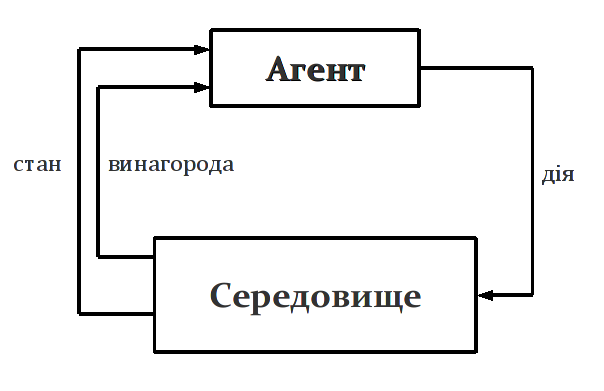
\includegraphics[width=0.8\textwidth]{agent_env_diagram.png}
\caption{Схема взаємодії агента та середовища}
\end{figure}
Схематично взаємодію агента та середовища представлено на рис.~\ref{agent_env_diagram}. В дискретний момент часу $t$ агент отримує стан середовища $s_t \in \mathcal{S}$, на основі цієї інформації він вибирає і здійснює певну дію $a_t \in \mathcal{A(s_t)}$, в результаті чого отримує певне значення миттєвої винагороди $r_t \in \mathbb{R}$ від середовища. Метою агента в такій системі є визначення для кожної можливої ситуації $s_t$ такої дії $a_t$, яка приводить до максимізації сумарної винагороди в довготерміновому періоді (\emph{очікуваного прибутку} $R_t$). Більш формально це можна визначити так. Потрібно визначити відображення $\pi:\mathcal{S}\times\mathcal{A} -> [0,1]$, яке називається \emph{стратегією}, таке, що $\pi(s, a)$ визначає ймовірність здійснення дії $a$ при перебуванні агента у стані $s$. В випадку детермінованої стратегії, $\pi(s,a) \in \{0,1\}$. Стратегія $\pi$ називається оптимальною, якщо для будь-якого стану послідовність дій, визначена нею, призводить до максимального очікуваного прибутку.

Визначимо більш точно поняття прибутку. Нехай, починаючи з часу $t$, агент отримує послідовність винагород $r_{t+1}, r_{t+2}, r_{t+3}, \ldots$. Тоді основною метою агента буде максимізація \emph{прибутку} $R_t$, де $R_t$ "--- це певна функція від послідовності винагород. В найпростішому випадку прибуток є сумою усіх винагород:

\begin{equation}
R_t = r_{t} + r_{t+1} + \cdots + r_T,
\end{equation}
де $T$ "--- кінцевий момент часу. Такий підхід до визначення прибутку підходить там, де можна природно визначити фінальний момент часу, тобто в таких системах, в яких взаємодія агента і середовища природньо розбивається на окремі послідовності (\emph{епізоди}), наприклад, партії в грі, проходи по лабіринту або будь-який інший вид повторюваних взаємодій.

Кожен епізод закінчується у \emph{кінцевому (термінальному) стані}, після якого відбувається встановлення стану системи в певний початковий стан з множини можливих початкових станів і розпочинається наступний епізод. Задачі, в яких взаємодія агента і середовища відбувається у вигляді послідовності епізодів, називаються \emph{епізодичними задачами}. В епізодичних задачах інколи розмежовують множину усіх нетермінальних станів системи $\mathcal{S}$ та множину усіх станів, включно з термінальними $\mathcal{S^+}$.

З іншого боку, не завжди можна здійснити природній поділ на епізоди, натомість взаємодія відбуваєть постійно без закінчення. Прикладом такої задачі може бути діяльність робота з великою тривалістю життєдіяльності. Такі задачі назвемо \emph{неперервними задачами}. В такому випадку кінцевий момент часу $T=\infty$, а сам прибуток, який ми намагаємося максимізувати може легко прямувати до нескінченості (наприклад, якщо на кожному кроці $r_t=1$). Щоб подолати ці труднощі, введемо дещо інше визначення прибутку.

Розглянемо додаткову концепцію "--- \emph{зважування}. Згідно з нею, агент намагаєтсья вибирати такі дії, щоб максимізувати суму зважених винагород, які він отримає в майбутньому. Зокрема, агент вибирає таку дію $a_t$, яка максимізує очікуваний \emph{зважений прибуток}:

\begin{equation}
R_t = r_{t} + \gamma r_{t+1} + \gamma^2 r_{t+2} + \cdots = \sum_{k=0}^{\infty}\gamma^k r_{t+k},
\end{equation}
де $\gamma$ "--- це параметр зважування, $0\leq\gamma\leq 1$.

Таке зважування дозволяє регулювати важливість певної винагороди, залежно від віддаленості її у часі. Так, винагорода, отримана через $k$ кроків у майбутньому, ``важитиме'' у $\gamma^k$ раз менше, ніж якби вона була отримана безпосередньо на поточному кроці. З такого визначення прибутку видно, що якщо $\gamma<1$, то ця нескінченна сума має скінченне значення, якщо послідовність $\left\{r_k\right\}$ "--- обмежена. Якщо $\gamma = 0$, то агент є ``недалекоглядним'' і буде дбати лише про максимізацію миттєвої винагороди. Його задачею в такому випадку буде вибір такої дії $a_t$, щоб максимізувати лише винагороду $r_{t}$. Якщо дія агента не здійснює вплив на майбутні винагороди (наприклад, якщо система має лише один стан), то такий підхід дійсно дасть змогу вивчити оптимальну стратегію, однак в більшості випадків це не так, тому максимізація лише миттєвої нагороди може призвести до того, що буде втрачено нагоду ``заробити'' більше в майбутньому, здійснивши на даному кроці дію, яка принесе не максимальну миттєву винагороду. З наближенням $\gamma$ до 1 агент надаватиме майбутнім винагородам все більшого значення: агент стає більш ``далекоглядним''. Надалі припускатимемо використання саме зваженого прибутку.

Існують різноманітні методи навчання агента. Однією з найбільш вивчених у літературі є група методів, які базуються на побудові \emph{функції корисності} $V(s)$, яка визначає максимальний очікуваний прибуток для стану $s$. Серед цих методів можна виділити три категорії алгоритмів:

\begin{itemize}
\item методи динамічного програмування;
\item методи Монте-Карло;
\item методи часової різниці.
\end{itemize}

В даній статті ми розглянемо алгоритми, що належать до останної категорії, оскільки перші дві не є надто практичними для більшості реальних застосувань. Для більш детального ознайомлення можна звернутися до \cite{SuttonBarto02}.

\subsection{Функція корисності}

Велика кількість алгоритмів навчання з підсиленням базується на оцінці \emph{функції корисності} "--- функції станів системи, що оцінює \emph{наскільки добре} для агента перебувати в заданому стані. Фраза ``наскільки добре'' визначається в термінах майбутніх очікуваного майбутнього прибутку. Очевидно, що майбутні винагороди залежать від того, які дії здійснювати, тобто від стратегії, тому ціннісна функція визначається з врахуванням певної стратегії.

Нагадаємо, що стратегія $\pi$ "--- це відображення кожного стану $s \in \mathcal{S}$ та кожної допустимої дії $a \in \mathcal{A}(s)$ на ймовірність $\pi(s,a)$ здійснення дії $a$, будучи в стані $s$. \emph{Корисністю} стану $s$ згідно стратегії $\pi$, $V^\pi(s)$,"--- це очікуваний прибуток, який можна отримати, якщо почати зі стану $s$ і діяти згідно стратегії $\pi$:
\begin{equation}
V^\pi(s) = E_\pi \Bigl\{ R_t \Big| s_t = s \Bigr \} = E_\pi \Biggl\{\sum_{k=0}^{\infty}\gamma^k r_{t+k+1} \Bigg| s_t=s \Biggr\},
\end{equation}
де $E_\pi{}$ позначає математичне очікування в випадку, якщо агент діє згідно стратегії $\pi$. Потрібно відмітити, що цінність термінального стану завжди рівна нулю. Назвемо функцію $V^\pi$ \emph{функцією корисності станів для статегії $\pi$}.

Аналогічно, визначимо корисність здійснення дії $a$ в стані $s$ згідно стратегії $\pi$, $Q^\pi(s,a)$, як очікуваний прибуток, отриманий в результаті перебування в стані $s$, здійснення дії $a$ та подальшому слідуванні стратегії $\pi$:
\begin{equation}
Q^\pi(s,a)=E_\pi \Bigl\{ R_t \Big| s_t=s, a_t=a \Bigr\} = E_\pi \Biggl\{\sum_{k=0}^{\infty}\gamma^k r_{t+k+1} \Bigg| s_t=s,a_t=a \Biggr\}.
\end{equation}
Назвемо функцію $Q^\pi$ \emph{функцією корисності дій для статегії $\pi$}.

Функції корисності $V^\pi$ та $Q^\pi$ можуть бути оцінені з досвіду. Наприклад, якщо агент притримується стратегії $\pi$ і підтримує середнє значення всіх прибутків, які були реально отримані, для кожного стану, в якому перебував агент, то середнє значення збіжиться до значення цінності для даного стану $V^\pi(s)$ за умови, що кількість перебувань в кожному зі станів прямує до нескінченності. Якщо зберігати середні значення окремо для кожної пари стан-дія, то таке ж твердження вірне і для функції $Q^\pi$. Такі методи оцінки цінових функцій називаються \emph{методами Монте-Карло}, тому що вони використовують усереднення по випадкових прикладах реальних прибутків. Проте, якщо кількість станів та можливих дій велика, це унеможливлює збереження середніх значень для кожного стану (пари стан-дія). В такому випадку можна застосувати інші методи, зокрема такі, що використовують апроксиматори функцій. Ми розглянемо їх дещо пізніше.

Фундаментальна властивість функцій корисності, яка використовується в навчанні з підсиленням і динамічному програмуванні,"--- це певне рекурсивне співвідношення, якому задовільняє функція корисності. Для будь-якої фіксованої стратегії $\pi$ та будь-якого стану $s$, наступне співвідношення завжди виконується:
\begin{eqnarray}
V^\pi(s) & = & E_\pi \Bigl\{R_t \Big| s_t = s \Bigr\} \nonumber\\
			& = & E_\pi \Biggl\{\sum_{k=0}^{\infty}\gamma^k r_{t+k+1} \Bigg| s_t = s \Biggr\} \nonumber\\
			& = & \sum_a \pi(s,a)\sum_{s'}\mathcal{P}^a_{ss'} \left[ \mathcal{R}^a_{ss'}+\gamma E_\pi \left\{\sum_{k=0}^{\infty}\gamma^k r_{t+k+2} \Bigg| s_{t+1} = s' \right\} \right] \nonumber\\
			& = & \sum_a \pi(s,a)\sum_{s'}\mathcal{P}^a_{ss'} \left[ \mathcal{R}^a_{ss'}+\gamma V^\pi(s') \right],
\label{Bellman_eq}
\end{eqnarray}
де $\mathcal{P}^a_{ss'}$ "--- це ймовірність переходу (transition probability) зі стану $s$ в стан $s'$ при виконанні дії $a$; $\mathcal{R}^a_{ss'}$ "--- очікувана винагорода, яка дається агенту при переході зі стану $s$ в стан $s'$ при виконанні дії $a$. В даній формулі неявно розуміється, що $s \in \mathcal{S}$, дії $a$ беруться з множини $\mathcal{A}(s)$, а $s' \in \mathcal{S}$ у випадку неперервної задачі або $s' \in \mathcal{S^+}$ "--- у випадку епізодичної задачі. Вказані ймовірності та очікувані винагороди визначають повну динаміку системи і на практиці зазвичай не відомі. Тому доводиться шукати методи, які б не потребували повних знань про систему.

Рівняння (\ref{Bellman_eq}) називається \emph{рівнянням оптимальності Белмана для $V^\pi$ (Bellman optimality equation for $V^\pi$)}. Воно відображає зв'язок між корисністю стану $s$ та корисністю станів $s'$, в які можна потрапити з $s$. Можна довести, що функція $V^\pi$ "--- єдиний розв'язок рівняння Белмана. Відмітимо також, що це рівняння "--- основа для багатьох методів обчислення, наближення та вивчення $V^\pi$.

\subsection{Оптимальні функції корисності}

Розв'язування задачі навчання з підсиленням означає, згрубша, знаходження такої стратегії, яка б давала великий прибуток в довгостроковій перспективі. Спробуємо визначити оптимальність стратегії наступним чином. Функції корисності визначають частковий порядок на множині усіх стратегій. Стратегію $\pi$ називатимемо \emph{кращою}, ніж стратегія $\pi '$, якщо її очікуваний прибуток більший або рівний від такого ж для стратегії $\pi '$ для усіх станів $s \in \mathcal{S}$:
\begin{equation}
\pi \geq \pi ' \Leftrightarrow \Bigl(\forall s \in \mathcal{S}\Bigr)\left\{ V^\pi(s) \geq V^{\pi '}(s) \right\}
\end{equation}

Завжди існує хоча б одна така стратегія, яка краща або рівна, ніж усі інші. Така стратегія називається \emph{оптимальною}. Хоча оптимальних стратегій може бути декілька, всіх їх будемо позначати як $\pi^*$. Усі оптимальні стратегії мають одну і ту ж функцію корисності станів, яка називається \emph{оптимальною функцією корисності станів} $V^*$:
\begin{equation}
V^* = \max_\pi V^\pi(s),\qquad \forall s \in \mathcal{S}.
\end{equation}

Оптимальні стратегії також мають одну і ту ж \emph{функцію корисності дій} $Q^*$:
\begin{equation}
Q^* = \max_\pi Q^\pi(s,a),\qquad \forall s \in \mathcal{S}, \forall a \in \mathcal{A}(s).
\end{equation}

Ми можемо також записати функцію $Q^*$ в термінах $V^*$:
\begin{equation}
Q^*(s,a) = E\left\{r_{t+1} + \gamma V^*(s_{t+1}) \Big| s_t=s, a_t=a \right\}.
\end{equation}

\subsection{Навчання з часовою різницею (TD-методи)}

Методи \emph{навчання з часовою різницею (temporal-difference, TD-навчання)} "--- це поєднання ідей методів Монте-Карло та динамічного програмування. TD-методи можуть, як і методи Монте-Карло, навчатися лише з досвіду, не потребуючи знання моделі динаміки середовища. З іншого боку, так само як і в методах динамічного програмування, TD-методи оновлюють свої оцінки частково на основі інших оцінок, не чекаючи закінчення епізоду.

\subsection{Стратегії вибору дій}
В усіх розглянутих алгоритмах потрібно на кожному кроці робити вибір дії, яку повинен здійснити агент. Це можна робити різними способами, проте, для збіжності стратегії до оптимальної, необхідною умовою є те, щоб кожна можлива дія була випробувана безліч раз при безмежній кількості ітерацій. Таку умову задовільняють так звані soft-стратегії, в яких ймовірність $\pi(s,a)>0,\ \forall \pi, \forall s \in \mathcal{S}, a \in \mathcal{A}(s)$.

Одним з найпростіших випадків soft-стратегії є $\varepsilon$-жадібна стратегія. В такій стратегії зазвичай вибирається дія, яка дає поточний максимум ціннісної функції, проте інколи, з ймовірністю $\varepsilon$, приймається рішення про здійснення довільної випадкової допустимої дії. Таким чином будь-яка не жадібна дія отримує ймовірність виконання, рівну $\frac{\varepsilon}{|\mathcal{A}(s)|}$, а жадібна дія, відповідно, $ 1 - \varepsilon + \dfrac{\varepsilon}{|\mathcal{A}(s)|}$.

Саме таку стратегію вибору дій було використано в цій роботі.

\subsection{Труднощі у випадку неперервного простору станів}

Якщо множина станів системи $\mathcal{S}$ дуже велика, як у випадку багатьох класичних ігор, або ж неперерва, то постає дуже важливе питання представлення функцій корисності. Існує багато варіантів вирішення цієї проблеми. І хоч ефективність кожного з методів сильно залежить від типу розв'язуваної задачі, одним з найбільш універсальних методів є лінійні та нелінійні апроксиматори фукнцій. При цьому лінійні апроксиматори, хоч і мають менші можливості, проте в більшості задач чудово справляються зі своїми завданнями і при цьому для випадку сумісного використання певних алгоритмів навчання з підсиленнями з лінійними апроксиматорами функцій були дані теоретичні гарантії збіжності до оптимальних стратегій при виконанні певних умов (\cite{Coulom2002}).

У випадку з нелінійними апроксиматорами, такими як штучні нейронні мережі, в силу їх більшої складності немає ніяких гарантій успішної збіжності до оптимальних стратегій. Більше того, для певних алгоритмів та задач було доведено, що використання нейромереж призводить до осциляції нейромережі (більш детальну інформацію можна знайти в \cite{SuttonBarto2002}). Тим не менше, нейромережі все ж таки успішно використовуються сумісно з різноманітними алгоритмами навчання з підсиленнями. Більше того, здатність нейромереж до узагальнення, дає можливість швидше навчати агента, оскільки визначивши вартість певного стану, вона певним чином наближає і вартості близьких станів. Таким чином потрібно менше ітерацій навчання для того, щоб функція корисності збіглася до оптимальної.

Як приклад одного з найуспішніших використань нейромереж у самонавчанні, можна навести програму TD-Gammon гри в нарди (backgammon), розроблену Gerald Tesauro (\cite{Tesauro1995}), яка в своїх останніх версіях грала на рівні з найкращими гравцями світу. Також успішні застосування нейромереж та методів навчання з підсиленнями можна знайти, наприклад, у \cite{Rummery1995} та \cite{Coulom2002}.

В даній роботі ми також використовували нейромережу як апроксиматор функцій і, як буде видно з результатів, досить успішно.

\subsection{Навчання з часовою різницею}
\subsection{Ускладнення задачі}
\section{Висновки}
\section{Література}
\begin{thebibliography}{99}
\bibitem{SuttonBarto02}{Sutton, R. S., Barto, A. G. 2002. Reinforcement Learning: An Introduction. A Bradford Book, The MIT Press, Cambridge, Massachusetts, London, England.}
\bibitem{Kun03}{Philippe Kunzle. Vehicle Control with Neural Networks "--- http://www.gamedev.net/reference/articles/article1988.asp}
\bibitem{Wik08}{Wikipedia. Control Theory "--- http://en.wikipedia.org/wiki/Control\_theory}
\end{thebibliography}

\end{document}
